\chapter{Background}
\label{chapter-background}
\begin{ChapAbstract}
This chapter provides an overview of the fundamental knowledge relevant to our thesis. We present a list of Computer Vision problems that play important roles in our proposed approach.
\end{ChapAbstract}

\section{Convolution Neural Network}
Convolutional neural network, also known as CNN or ConvNet, was introduced by Yann LeCun et al.~\cite{LeCun-NC1989-Backpropagation} to understand and explain visual data such as images. A digital image contains pixels arranged in a grid to represent information about colour, brightness, texture, etc. The CNN network is inspired by how the human visual system processes data on each receptive field. CNN is commonly used for extracting feature maps from images containing information about the relationship between pixels. This information can be used as the input for the downstream tasks: image classification, object detection, etc.

\subsection{Convolution Layer}
The convolution Layer is the core block of a CNN. It extracts information from the input through matrix multiplications. Specifically, it performs multiplications between a set of learnable parameters, known as a kernel, and the corresponding matrix bounded by the receptive fields. In mathematics, the convolution between two functions~\cite{Rudin-McGrawHill1991-Functional}, $f, g: \mathbb{R}^d \rightarrow \mathbb{R}$ is defined as:

\begin{equation}
    (f \ast g)(x) = \int f(z)g(x - z)dz,
\end{equation}

For two-dimensional matrices, we have the formula:
\begin{equation}
    (f \ast g)(i, j) = \sum_{a}^{A-1}\sum_{b}^{B-1}f(a, b)g(i - a, j - b),
\end{equation}
Where f is the kernel and g is the input image with size $A \times B$. An illustration of the formula is shown in~\autoref{fig:chapter2-convolution-compute}.

\begin{figure}[h!]
    \centering
    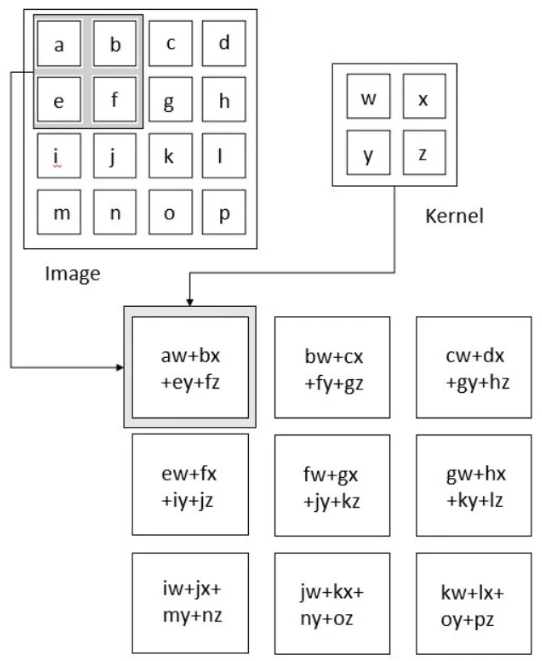
\includegraphics[width=0.5\linewidth]{content/resources/images/background/convolution-compute.png}
    \caption{Convolution operation (Source: Deep Learning~\cite{Goodfellow-MIT2016-DL}).}
    \label{fig:chapter2-convolution-compute}
\end{figure}

Visually, the convolution window (kernel) is slid over all the height and width of images to compute the result at each spatial position. However, with this method, we can only shift the kernel pixel by pixel, leading to high computational costs when the input size is large. Stride and padding are techniques applied in convolution for computational efficiency and to control the downsampling rate. Stride is the number of elements that the window moves at a time. It enables to capture a larger receptive field. Padding is the extra pixels added around the border of the input before performing the convolution operation to keep the input dimensions after convolution. If we have an input of size $W_{in} \times H_{in}$ and kernel of size $F$ with stride $S$ and padding $P$, then the size of output is $W_{out} \times H_{out}$ (as illustrated in~\autoref{fig:chapter2-convolution}):
\begin{equation}
    \begin{cases} 
        W_{out} = \dfrac{W_{in} - F + 2P}{S} + 1 \\ 
        H_{out} = \dfrac{H_{in} - F + 2P}{S} + 1 
    \end{cases}.
\end{equation}

\begin{figure}[h!]
    \centering
    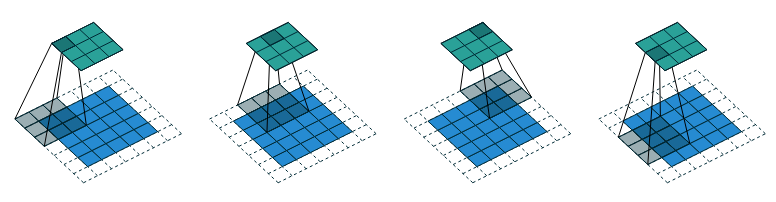
\includegraphics[width=\linewidth]{content/resources/images/background/convolution.png}
    \caption{Two-dimensional convolution ($F=3, S = 2, P = 1$) with input of size $W_{in} = H_{in} = 5$. After sliding the kernel over all the input, we get the output with size  $W_{out} = H_{out} = 3$ (Source: A guide to convolution arithmetic for deep learning~\cite{Dumoulin-ArXiv2016-Guide}).}
    \label{fig:chapter2-convolution}
\end{figure}

\subsection{Pooling Layer}
The pooling layer is commonly inserted between successive convolution layers to reduce the spatial size of the feature maps by aggregating information from local regions. This help decreases the number of parameters and computation and prevents overfitting. The pooling operation uses a window slid over all the input to compute an output for each region. Unlike the convolution layer, the window of the pooling layer contains no parameters. Instead, the output of the regions in the window is determined by a unified function, such as the maximum or the average of the neighbours in the pooling window area. 

The pooling operation is processed independently on every depth slice of the input. If we have an input of size $W_{in} \times H_{in} \times D_{in}$ and a pooling window with size $F$ and stride $S$, the pooling layer produces an output of size $W_{out} \times H_{out} \times D_{out}$ ($D_{in}, D_{out}$ are the depth size) where:
\begin{equation}
    \begin{cases} 
        W_{out} = \dfrac{W_{in} - F}{S} + 1 \\ 
        H_{out} = \dfrac{H_{in} - F}{S} + 1 \\
        D_{out} = D_{in}
    \end{cases}.
\end{equation}

\begin{figure}[h!]
    \centering
    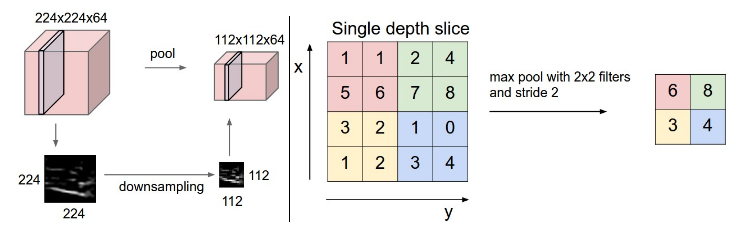
\includegraphics[width=\linewidth]{content/resources/images/background/maxpool.png}
    \caption{Pooling operation downsample by applying the kernel to each slice. \textbf{Left}: Appling pooling operation with $F = 2, S = 2$ reduces the input size from $224x \times 224 \times 64$ to  $112x \times 112 \times 64$. \textbf{Right}: Illustration of the max pooling with $F = 2, S = 2$, which preserves the maximum value in adjacent pixels (Source: CS231n: Deep Learning for Computer Vision~\cite{Stanford-CS231n}).}
    \label{fig:chapter2-maxpool}
\end{figure}


\section{Attention and Transformer}
\subsection{Self-attention}
Self-attention is a sequence-to-sequence operation: the input is a sequence of vectors that goes in, and the output is also a sequence of vectors. This operation is proposed in the paper "Attention is all you need" \cite{Vaswani-NeurIPS2017-Attention}. We denote the input vectors as $x_1, x_2, ..., x_t$ and the corresponding output vectors $y_1, y_2, ..., y_t$. All vectors have dimension k.

The self-attention operation takes a weighted average over all the input vectors, as in \autoref{eq:self-attention}. The weight values can be derived from the input vectors themselves, which is why this operation is called self-attention. \autoref{eq:self-attention-weight} shows the simplest option, the dot product.

\begin{equation}
y_i = \sum_{j} w_{ij} x_j,
\label{eq:self-attention}
\end{equation}

\begin{equation}
w_{ij} = \dfrac{exp(w'_{ij})}{\sum_{j} exp(w'_{ij})},
\end{equation}

\begin{equation}
w'_{ij} = x^T_ix_j.
\label{eq:self-attention-weight}
\end{equation}

Modern deep-learning architectures further improve this operation by adding three $k x k$ learnable matrices, denoted as $W_q$, $W_k$, and $W_v$. We apply these matrices as the linear transformations of the input vectors $x_i$. \autoref{eq:self-attention-modern} shows the specific formula.

\begin{equation}
y_i = \sum_{j} w_{ij} (W_v x_j),
\label{eq:self-attention-modern}
\end{equation}

\begin{equation}
w_{ij} = \dfrac{exp(w'_{ij})}{\sum_{j} exp(w'_{ij})},
\end{equation}

\begin{equation}
w'_{ij} = (W_qx_i)^T(W_kx_j).
\end{equation}


\subsection{Multi-head Self-attention}
Using a single self-attention operation, each input vector $x_j$ can only influence every output vector $y_i$ in a fixed way, depending on the transformation matrices $W$. To tackle this problem, Vaswani et al.\cite{Vaswani-NeurIPS2017-Attention} combine multiple self-attention mechanisms (indexed with $r$), which involve learning different matrices $W^r_k, W^r_q,$ and $W^r_v$. These are called attention heads $h$. Each attention head gives different output vectors $y^r_i$. These vectors are concatenated along all attention heads and passed through a linear transformation to reduce the dimension to $k$. \autoref{fig:chapter2-multihead} illustrates how multi-head self-attention works.

\begin{figure}[h!]
    \centering
    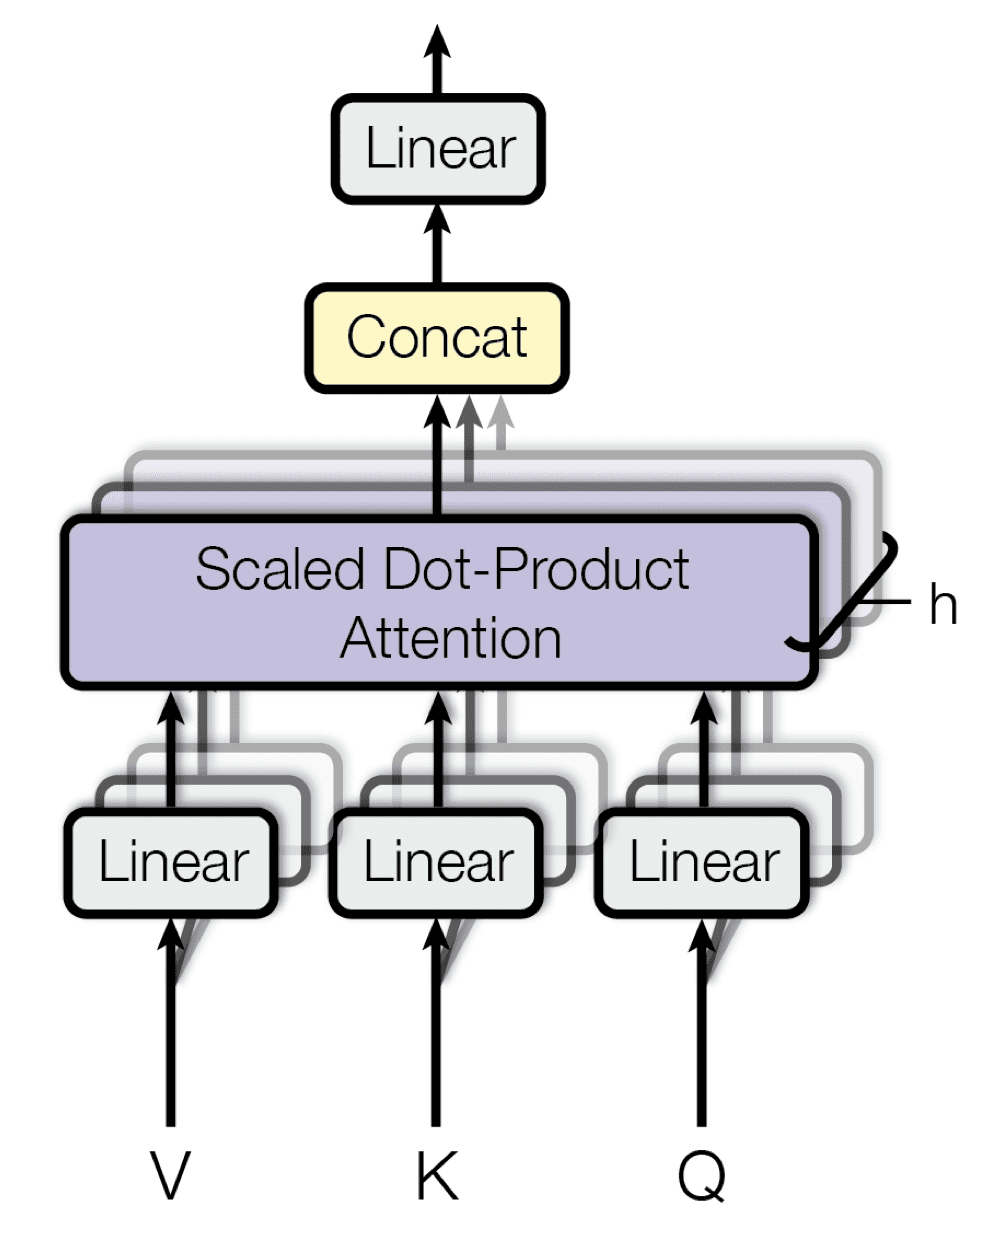
\includegraphics[width=0.3\linewidth]{content/resources/images/background/multihead.png}
    \caption{Multi-head self-attention mechanism (Source: Attention is all you need~\cite{Vaswani-NeurIPS2017-Attention}).}
    \label{fig:chapter2-multihead}
\end{figure}

However, this approach has one drawback, which takes $h$ times slower as the number of heads increases. Multi-head self-attention solves this problem by slicing the input vectors into $h$ chunks and performing the multi-head self-attention on each chunk. For example, if we have 640-dimension input vectors and 16 attention heads, we need to slice each input vector into 16 chunks of 40 dimensions. 

\subsection{Transformers}

Each transformer's block is built upon a multi-head self-attention block, followed by a normalization layer, a single multi-layer perception applied independently to each input vector, and another normalisation layer. Residual connections are added before both normalizations. \autoref{fig:chapter2-transformer} shows the architecture of a Transformers block.

\begin{figure}[h!]
    \centering
    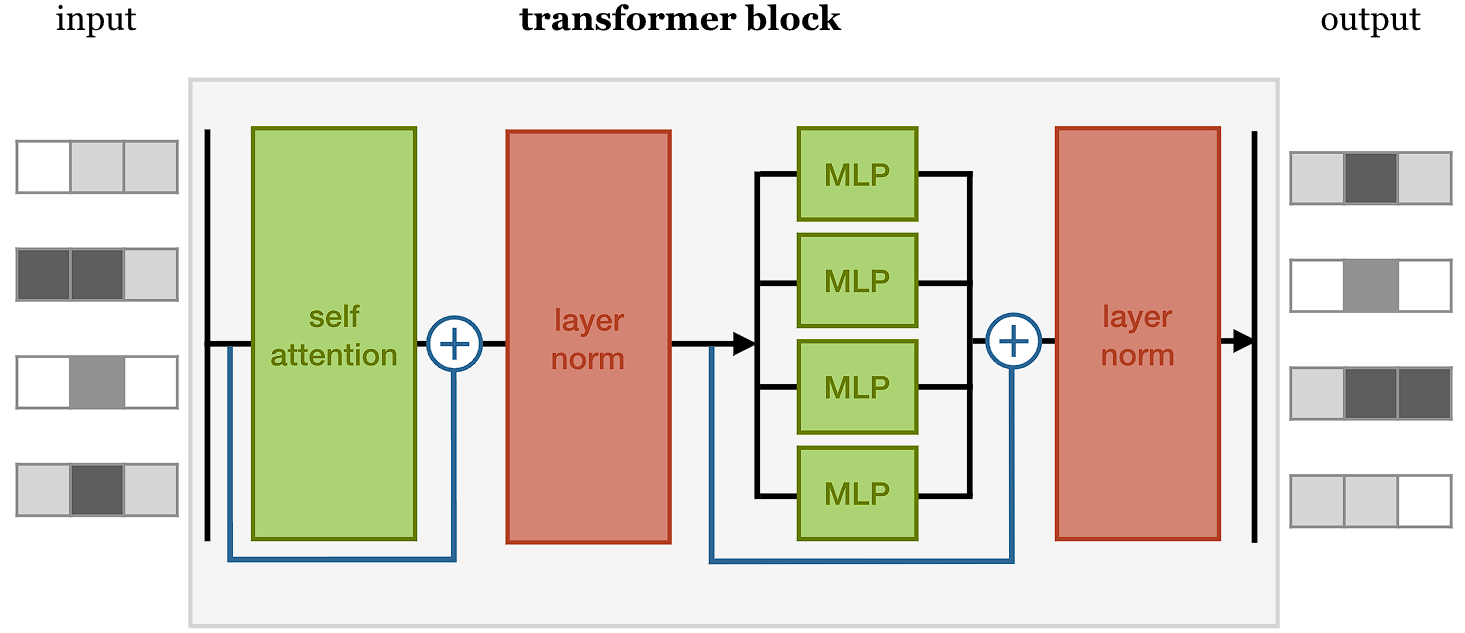
\includegraphics[width=\linewidth]{content/resources/images/background/transformers.PNG}
    \caption{Transformers block architecture (Source: Transformers from scratch~\cite{web-transform-from-scratch}).}
    \label{fig:chapter2-transformer}
\end{figure}

A \textbf{Transformers block} can produce a sequence of vectors given a sequence of vectors, so it is also a sequence-to-sequence model. Modern deep-learning architectures~\cite{Vaswani-NeurIPS2017-Attention, Devlin-ArXiv2018-BERT} utilize this characteristic and apply multiple Transformers blocks sequentially, called \textbf{Transformers Encoder}, to improve the overall performance.

Especially, in BERT~\cite{Devlin-ArXiv2018-BERT}, the author uses a special vector \textit{<CLS>} as the first input vector. The Transformers Encoder is trained so that the first output vector captures the semantics of the whole sequence of input vectors (\autoref{fig:chapter2-bert}). After being proposed, this approach is widely adopted for downstream tasks, such as classification, which require one embedding representing the whole input.

\begin{figure}[h!]
    \centering
    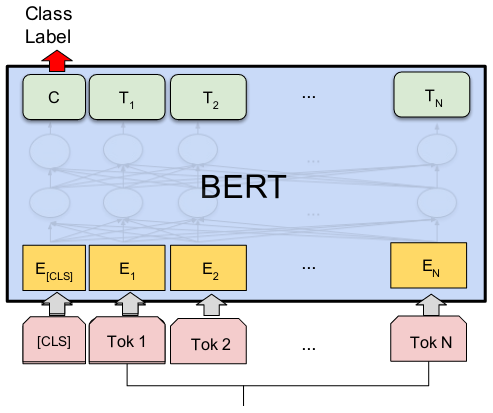
\includegraphics[width=0.7\linewidth]{content/resources/images/background/bert_class.png}
    \caption{BERT \textit{<CLS>} vector (Source: Text classification using BERT~\cite{web-bert}).}
    \label{fig:chapter2-bert}
\end{figure}
